\section{Parameter Choices}\label{sec:param_choices}
The critical parameters for \mt are $K$ and $h$, where parameter $K$ is used by the K-means during orientation clustering while parameter $h$ which is used by the hierarchical clustering.
K denotes the number of major fiber bundle directions. This is known a priori or can be estimated by considering the weaving pattern. 
\begin{figure}[tb]
	\centering
	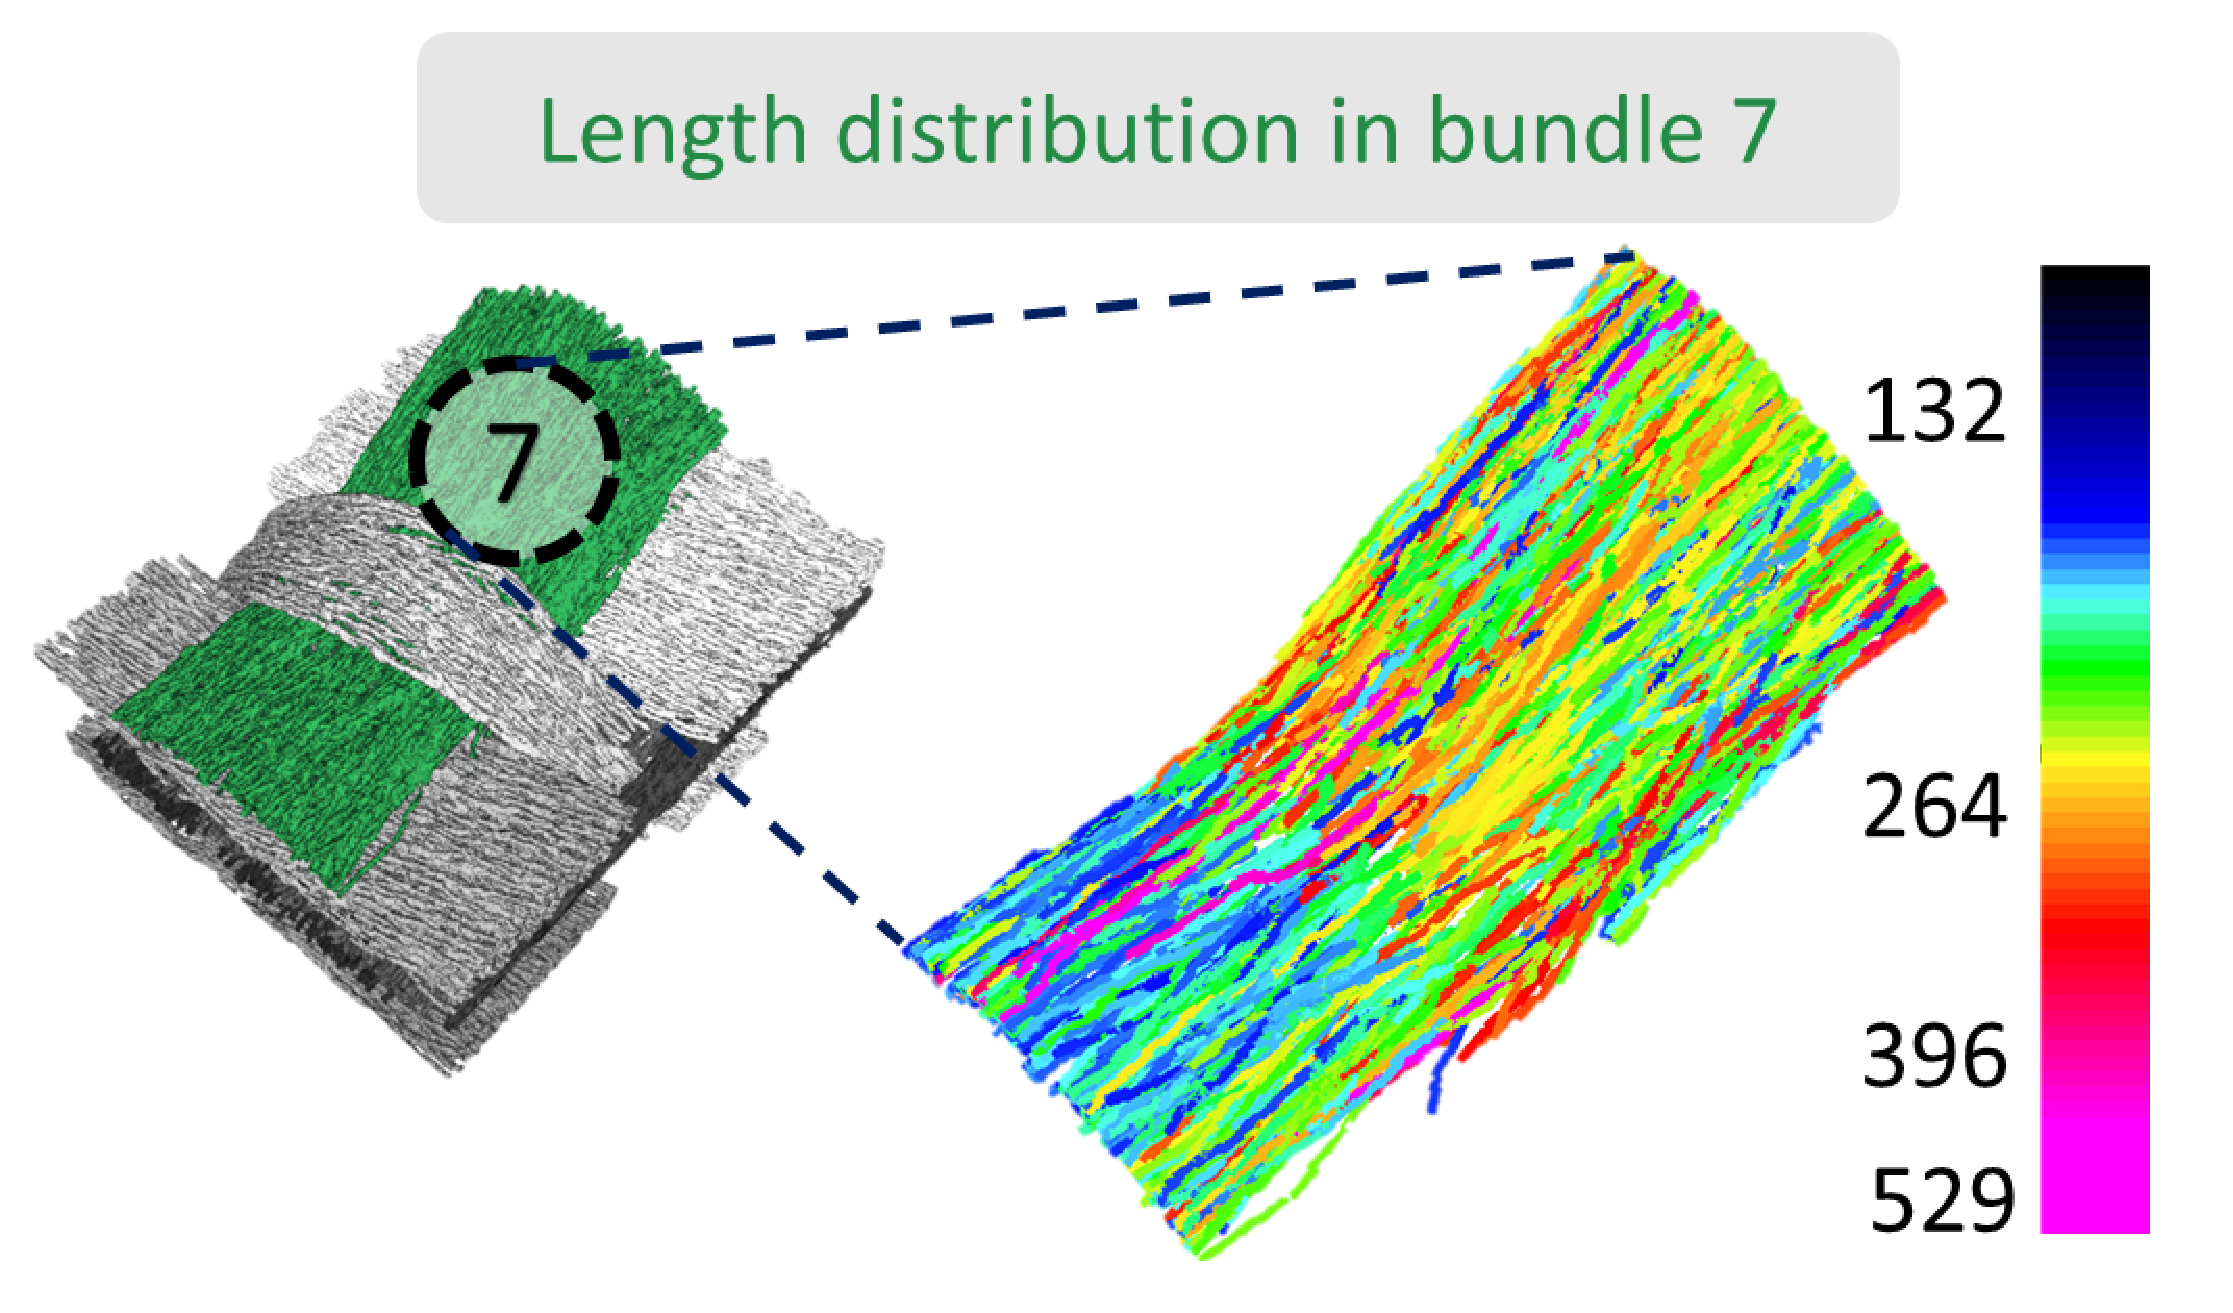
\includegraphics[width=0.8\linewidth]{images/lengthDistribution.eps}
	\caption{(a) Length distribution of individual \mt for a particular bundle (unit for length is grid cube edge length:  $2\mu m$).}
	\label{fig:length_distribution}
\end{figure}
\begin{figure}[tb]
	\centering
	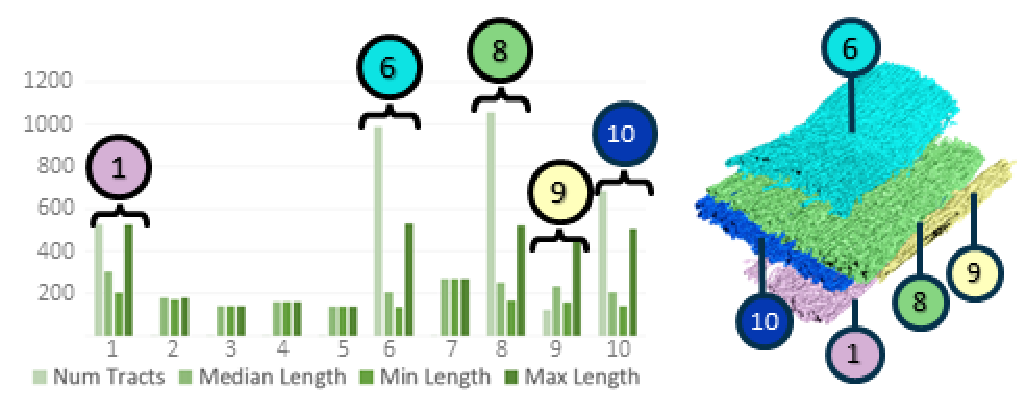
\includegraphics[width=\linewidth,  trim = 0mm 0mm 0mm 00mm, clip]{images/figure9_AMA.eps}
	\caption{Number of \mt and median, minimum and maximum length of an individual MetaTracts in the orientation cluster Figure~\ref{fig:orientation_clustering}\brac{d} when clustered into 10 clusters. The unit for the MetaTracts length is the grid cube length. The labeled clusters 2, 3, 4, 5 and 7 have a cardinality less than 10 and are removed. }
	\label{fig:len_dist_crop16} 
\end{figure}
Figure~\ref{fig:len_dist_crop16} shows the number of \mt in each cluster when the orientation cluster 1 (Figure ~\ref{fig:orientation_clustering}\brac{a}) is hierarchically clustered into ($h$) 10 clusters. It also shows the minimum, maximum and median length of the MetaTracts in each of the resulting clusters. The ground truth was five separate fiber bundles. We observe that the major fiber bundles remain well separated in accordance with our ground truth and the small clusters (clusters 2, 3, 4, 5 and 7) have very few elements and can be easily discarded. Thus we see that our framework is robust to the choice of parameter $h$ for hierarchical clustering. This is an appealing trait of the proximity based hierarchical clustering, thus providing good results even when exact $h$ might be unknown. The robustness to parameter variation also reinforces our two-step approach to clustering. 


The following parameters were fixed for all the tests. We set the reliable Hessian threshold $R_{H}$ to be 0.3. A $R_{H}$ of 0.0 would mean all points have reliable local orientation which would cause spurious MetaTracts detection. A very high $ R_{H}$ would lead to a decline in number of MetaTracts produced. Coefficients $\alpha$ and $\beta$ in $R_{H}$ are as explained in Frangi et al.~\cite{Frangi1998} and set to 0.5. The length and the radius parameters for the cylinders of MetaTracts decide how coarse our approximation of the fiber bundles are. These are dependent on the underlying fiber characteristic and the weaving pattern. Larger cylinders will handle noisy local orientation better as it inspects a larger number of candidate points to extend the fiber. We used 10 and 2 for length and radius (measured in grid voxel size), respectively for all tests.  
A simpler geometry (e.g., D2) was experimentally found to handle larger cylinders better. $\eta$ in Sec.~\ref{subsec:dist_clustering} decides how quickly the hierarchical clustering converges, experimentally values 0.3 to 0.6 removed $1.2\% - 5\%$ of fibers (total number of fibers $\sim$10000) and gave similar results. We set $n$ the number of sampled \mt to 10.000 for all our test cases. Parameter $n$ intuitively acts as ``resolution" for the MetaTracts. Large $n$ captures the features better and generates smoother fiber bundles. 

$\alpha$ and $\beta$ in equation~\ref{eqn:algo_1} decide how quickly the value of the factor decays; we have used integer values between [7-10] and half the length of an individual cylinder respectively. Our number of fiber bundle directions is limited. Thus even for small $m$ (cardinality of lower dimension in orientation clustering), the distinction between the orientation clusters is preserved quite well. We compared $m=3,...,7$ experimentally without any change in results. 
\section{Limitations}\label{sec:limitations}
A key assumption of the method is ``connectivity'' (Sec.~\ref{sec:char_data}).
If the ``connectivity'' criteria is not fulfilled due to noise in the image, then the generated MetaTracts will be inaccurate. 
The clustering process also assumes that the fiber bundles have a minimum width.
\section{Conclusions and Future Work}\label{subsec:conclusions}
In this paper, we introduce a framework to extract and visualize fiber bundles in composite materials. We show that our framework works at comparatively low resolution and with dense fiber arrangements (when extracting single fibers might not be possible). It handles complex fiber patterns such as ``cross overs'' and ``braiding''.
In addition, we demonstrated a tool to interactively investigate and analyze voxelized fiber bundles generated with the MetaTracts approach.

In future, we plan to increase the precision of the extractions, include uncertainty based visualization to better portray the surface of separations and speed up extraction times.
